\section*{Ordinary Differential Equations}
In ordinary calculus, we usually want to find values of a function given the rate of change. For example, let $f(t)$ denote the position of a particle at time $t$, and that we are given the function for the rate of change as
\begin{align*}
df(t) = C\big(f(t), t\big)dt
\end{align*}
Then given the initial condition $f(0)=x_0$, we can approximate the function for some small increment of $t$ using Euler's method
\begin{align*}
f(t + \Delta t) = f(t) + C \big(f(t), t \big)\Delta t
\end{align*}
\begin{figure}[h!]
    \centering
    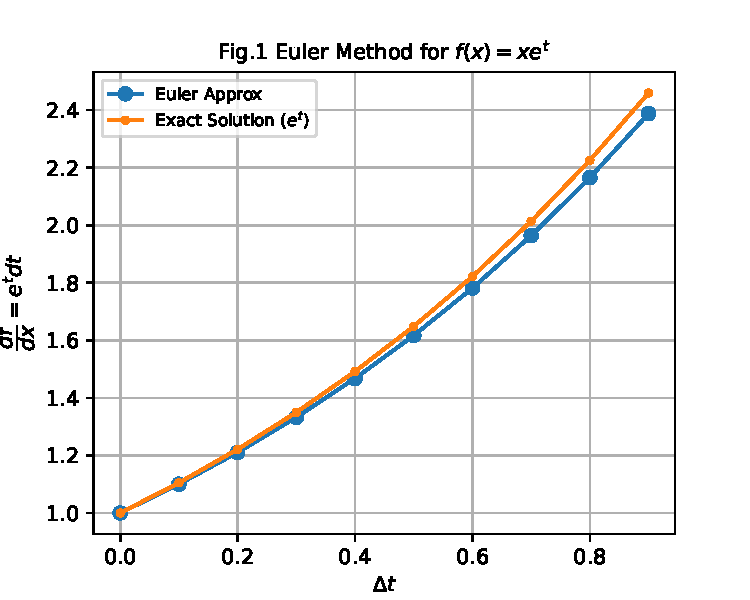
\includegraphics[width=0.5\textwidth]{figures/euler_method.pdf}
    \vspace{-25pt}
    \caption{\small Euler Method}
    \label{fig:fig_1}
\end{figure}
Euler's method is a simple way to approximate the ordinary differential equation. By taking smaller step sizes of $\Delta t$ we could reach closer approximations to the exact value of the function. On the other hand, the method to approximate a stochastic differential equation is by using the \textbf{Euler-Maruyama} method.